\documentclass[10pt,aspectratio=149]{beamer}
\usecolortheme{Calm}
\usetheme{Calm}
\usepackage{amsmath}
\usepackage{pgfplots}
\pgfplotsset{compat=1.18}
\usepackage{pgfplotstable}
\usepackage[utf8]{inputenc}
\usepackage{hyperref}
\RequirePackage[absolute,overlay]{textpos}
%\usepackage[sfdefault]{cabin}
%\usepackage[T1]{fontenc}
%\setlength{\TPHo{}rizModule}{\paperwidth}
%\setlength{\TPVertModule}{\paperheight}
%\definecolor{OQEdarkblue}{HTML}{046085}


\defbeamertemplate*{background canvas}{bg}
{%
  \color{lightgray!40}\vrule width\paperwidth height\paperheight% added bg color
}

% Centered, larger display equation
\newcommand{\keyeq}[1]{%
  \begin{center}
    \Large$\displaystyle #1$
  \end{center}%
}

% Same style, for a system of equations aligned on "="
% (rows separated by \\, each row written as LHS &= RHS)
\newcommand{\keyeqs}[1]{%
  \begin{center}
    \normalsize$\displaystyle
    \begin{aligned}
    #1
    \end{aligned}
    $
  \end{center}%
}

%------------------------------

\author{Dominique Gravel}
\title{Metapopulation dynamics}
\date{August 24th, 2026}
\institute{Université de Sherbrooke \\ Summer school in biodiversity modelling}

%------------------------------
% TITLE SLIDE
%------------------------------

\usebackgroundtemplate
{
  
\includegraphics[width=\paperwidth,height=\paperheight]{bg}%
}

\begin{document}

	\begin{frame}[plain]
		\titlepage
	\end{frame}

%------------------------------
% INTRODUCTION
%------------------------------

\begin{frame}

    \begin{center}
        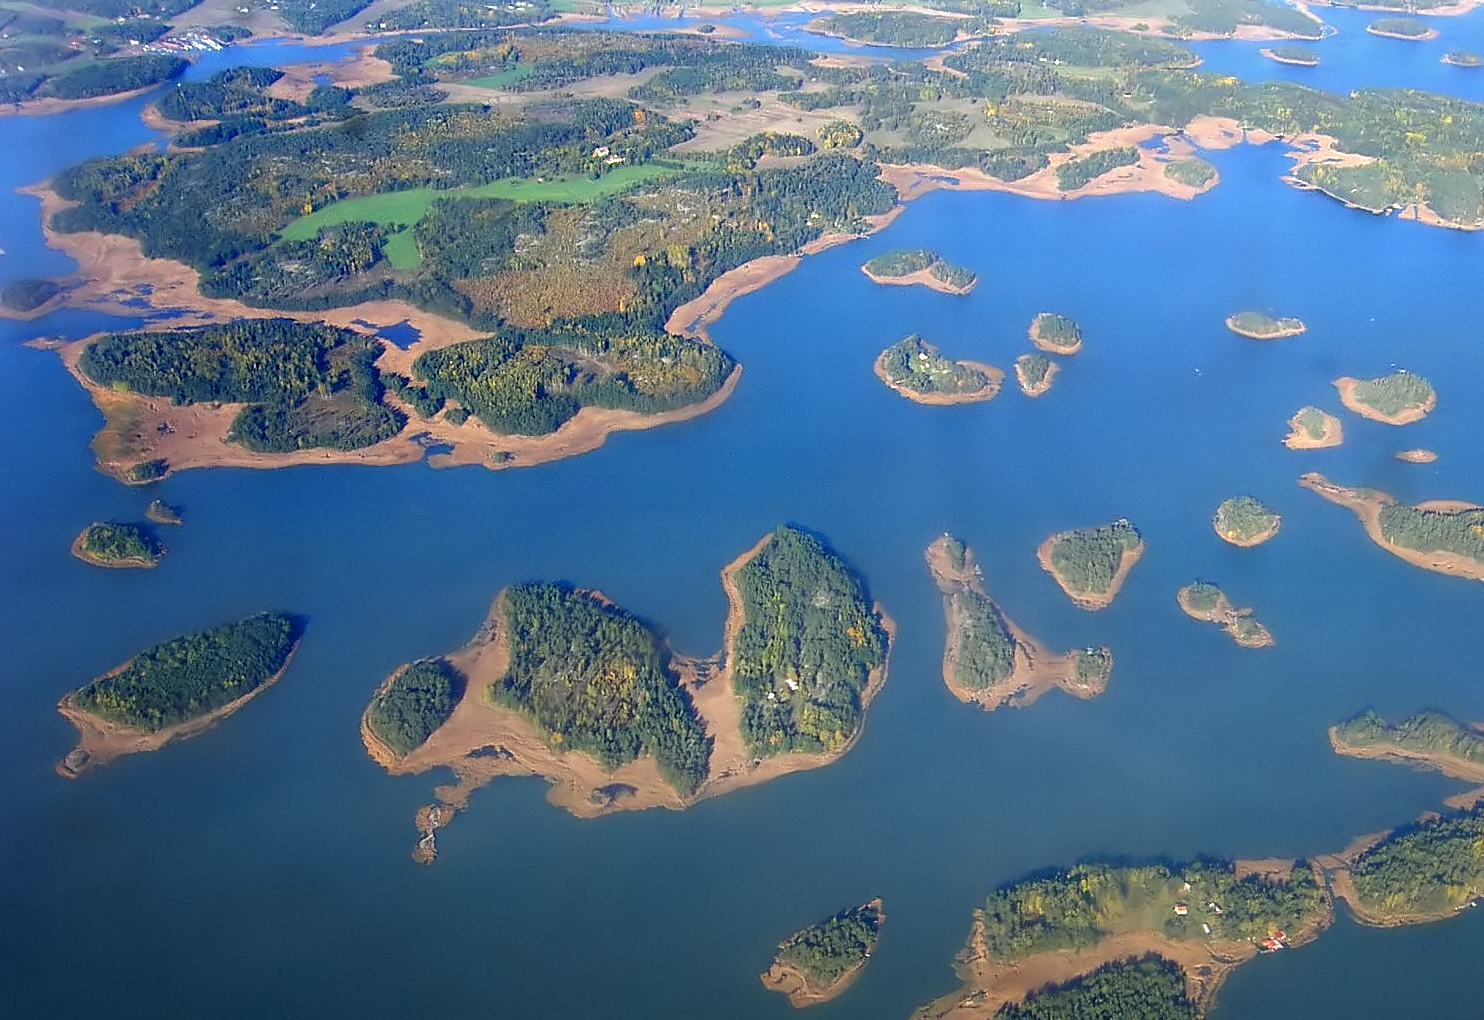
\includegraphics[height=0.7\textheight]{Figs/archipelago}
    \end{center}

\end{frame}

%------------------------------

\begin{frame}

    \begin{center}
        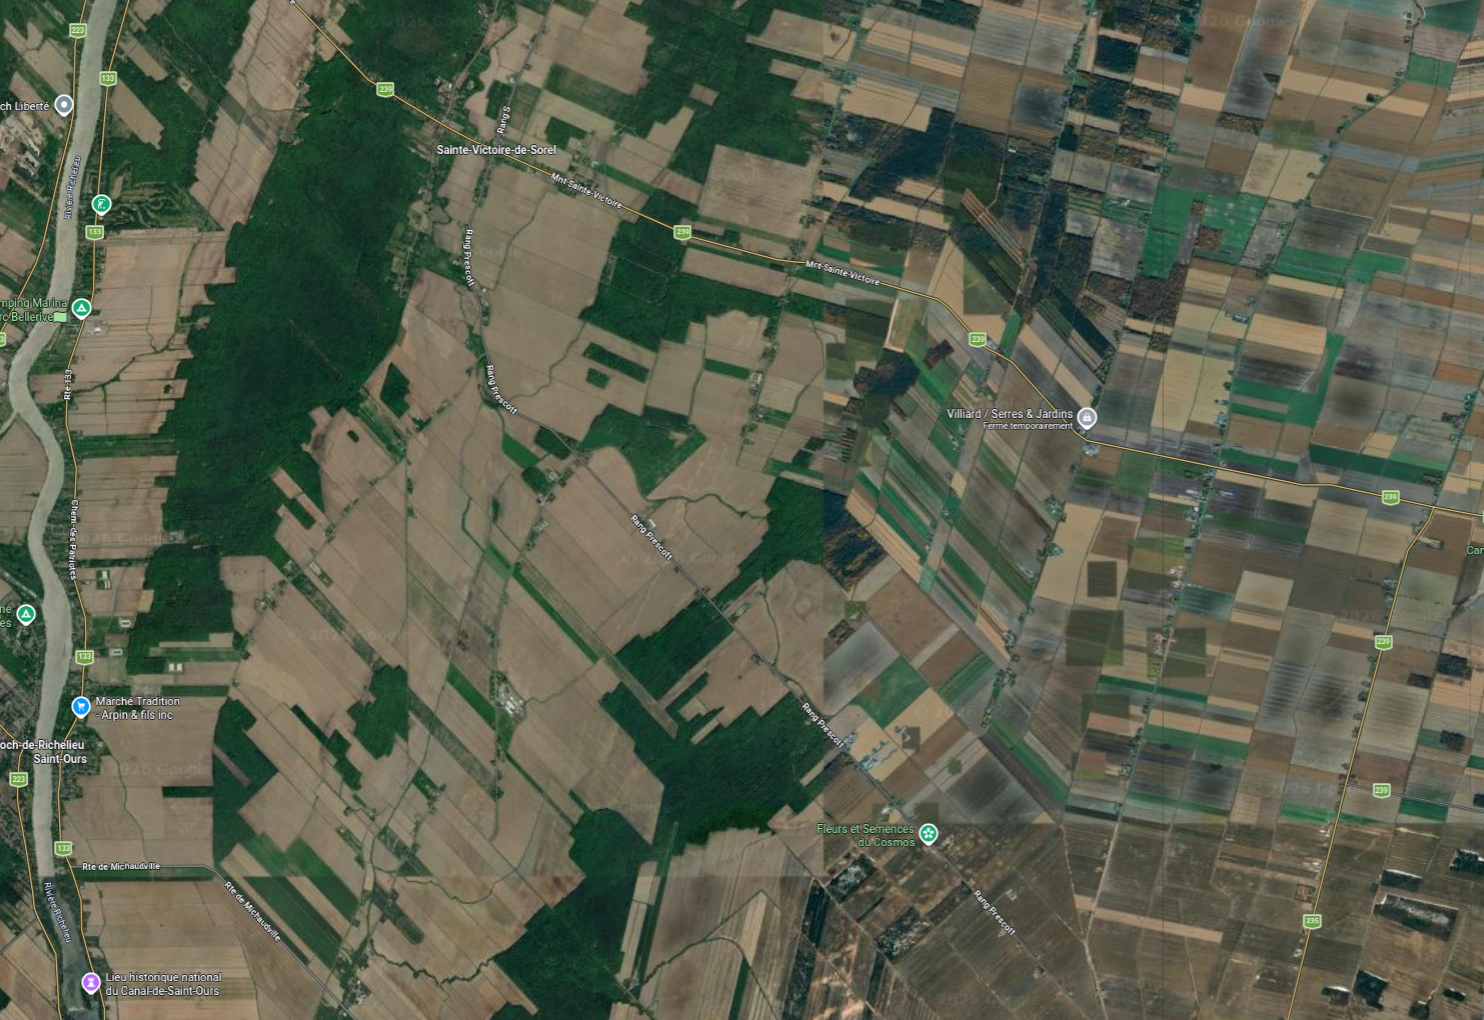
\includegraphics[height=0.7\textheight]{Figs/forest_landscape}
    \end{center}

\end{frame}

%------------------------------

\begin{frame}

    \begin{center}
        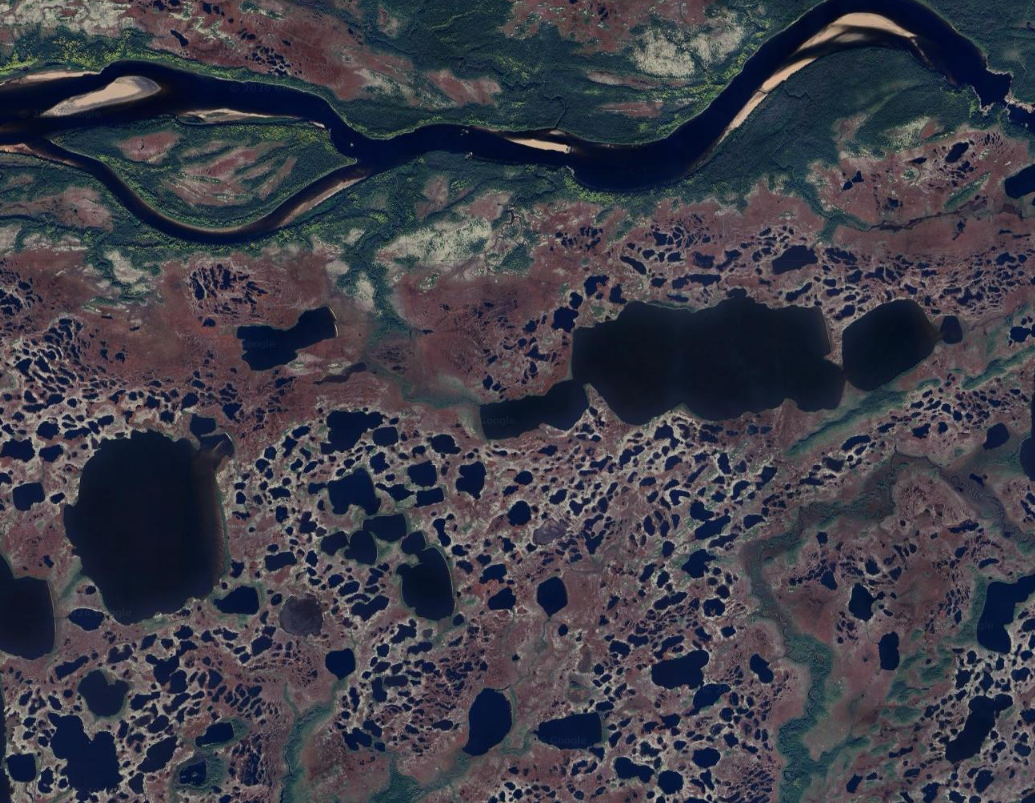
\includegraphics[height=0.7\textheight]{Figs/ponds}
    \end{center}

\end{frame}

%------------------------------

\begin{frame}

    \begin{center}
        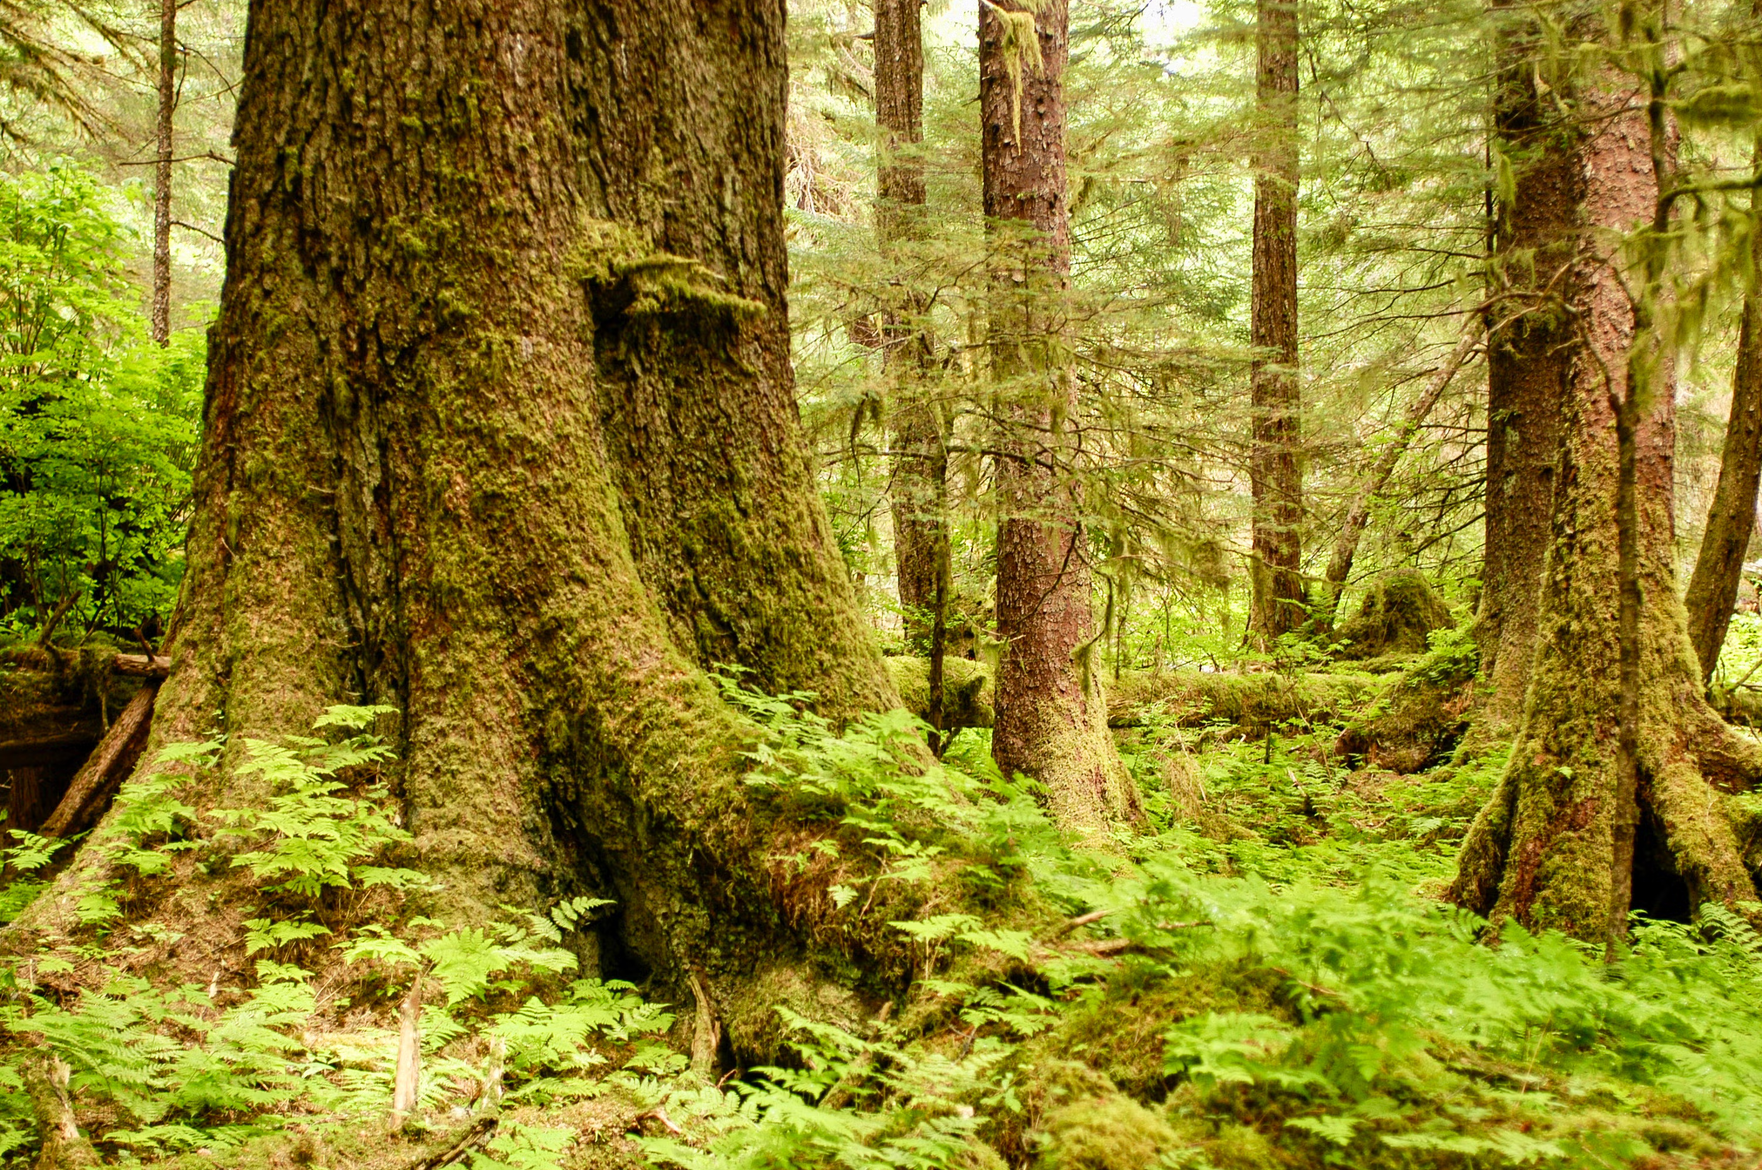
\includegraphics[height=0.7\textheight]{Figs/trees}
    \end{center}

\end{frame}

%------------------------------

\begin{frame}

    \begin{center}
        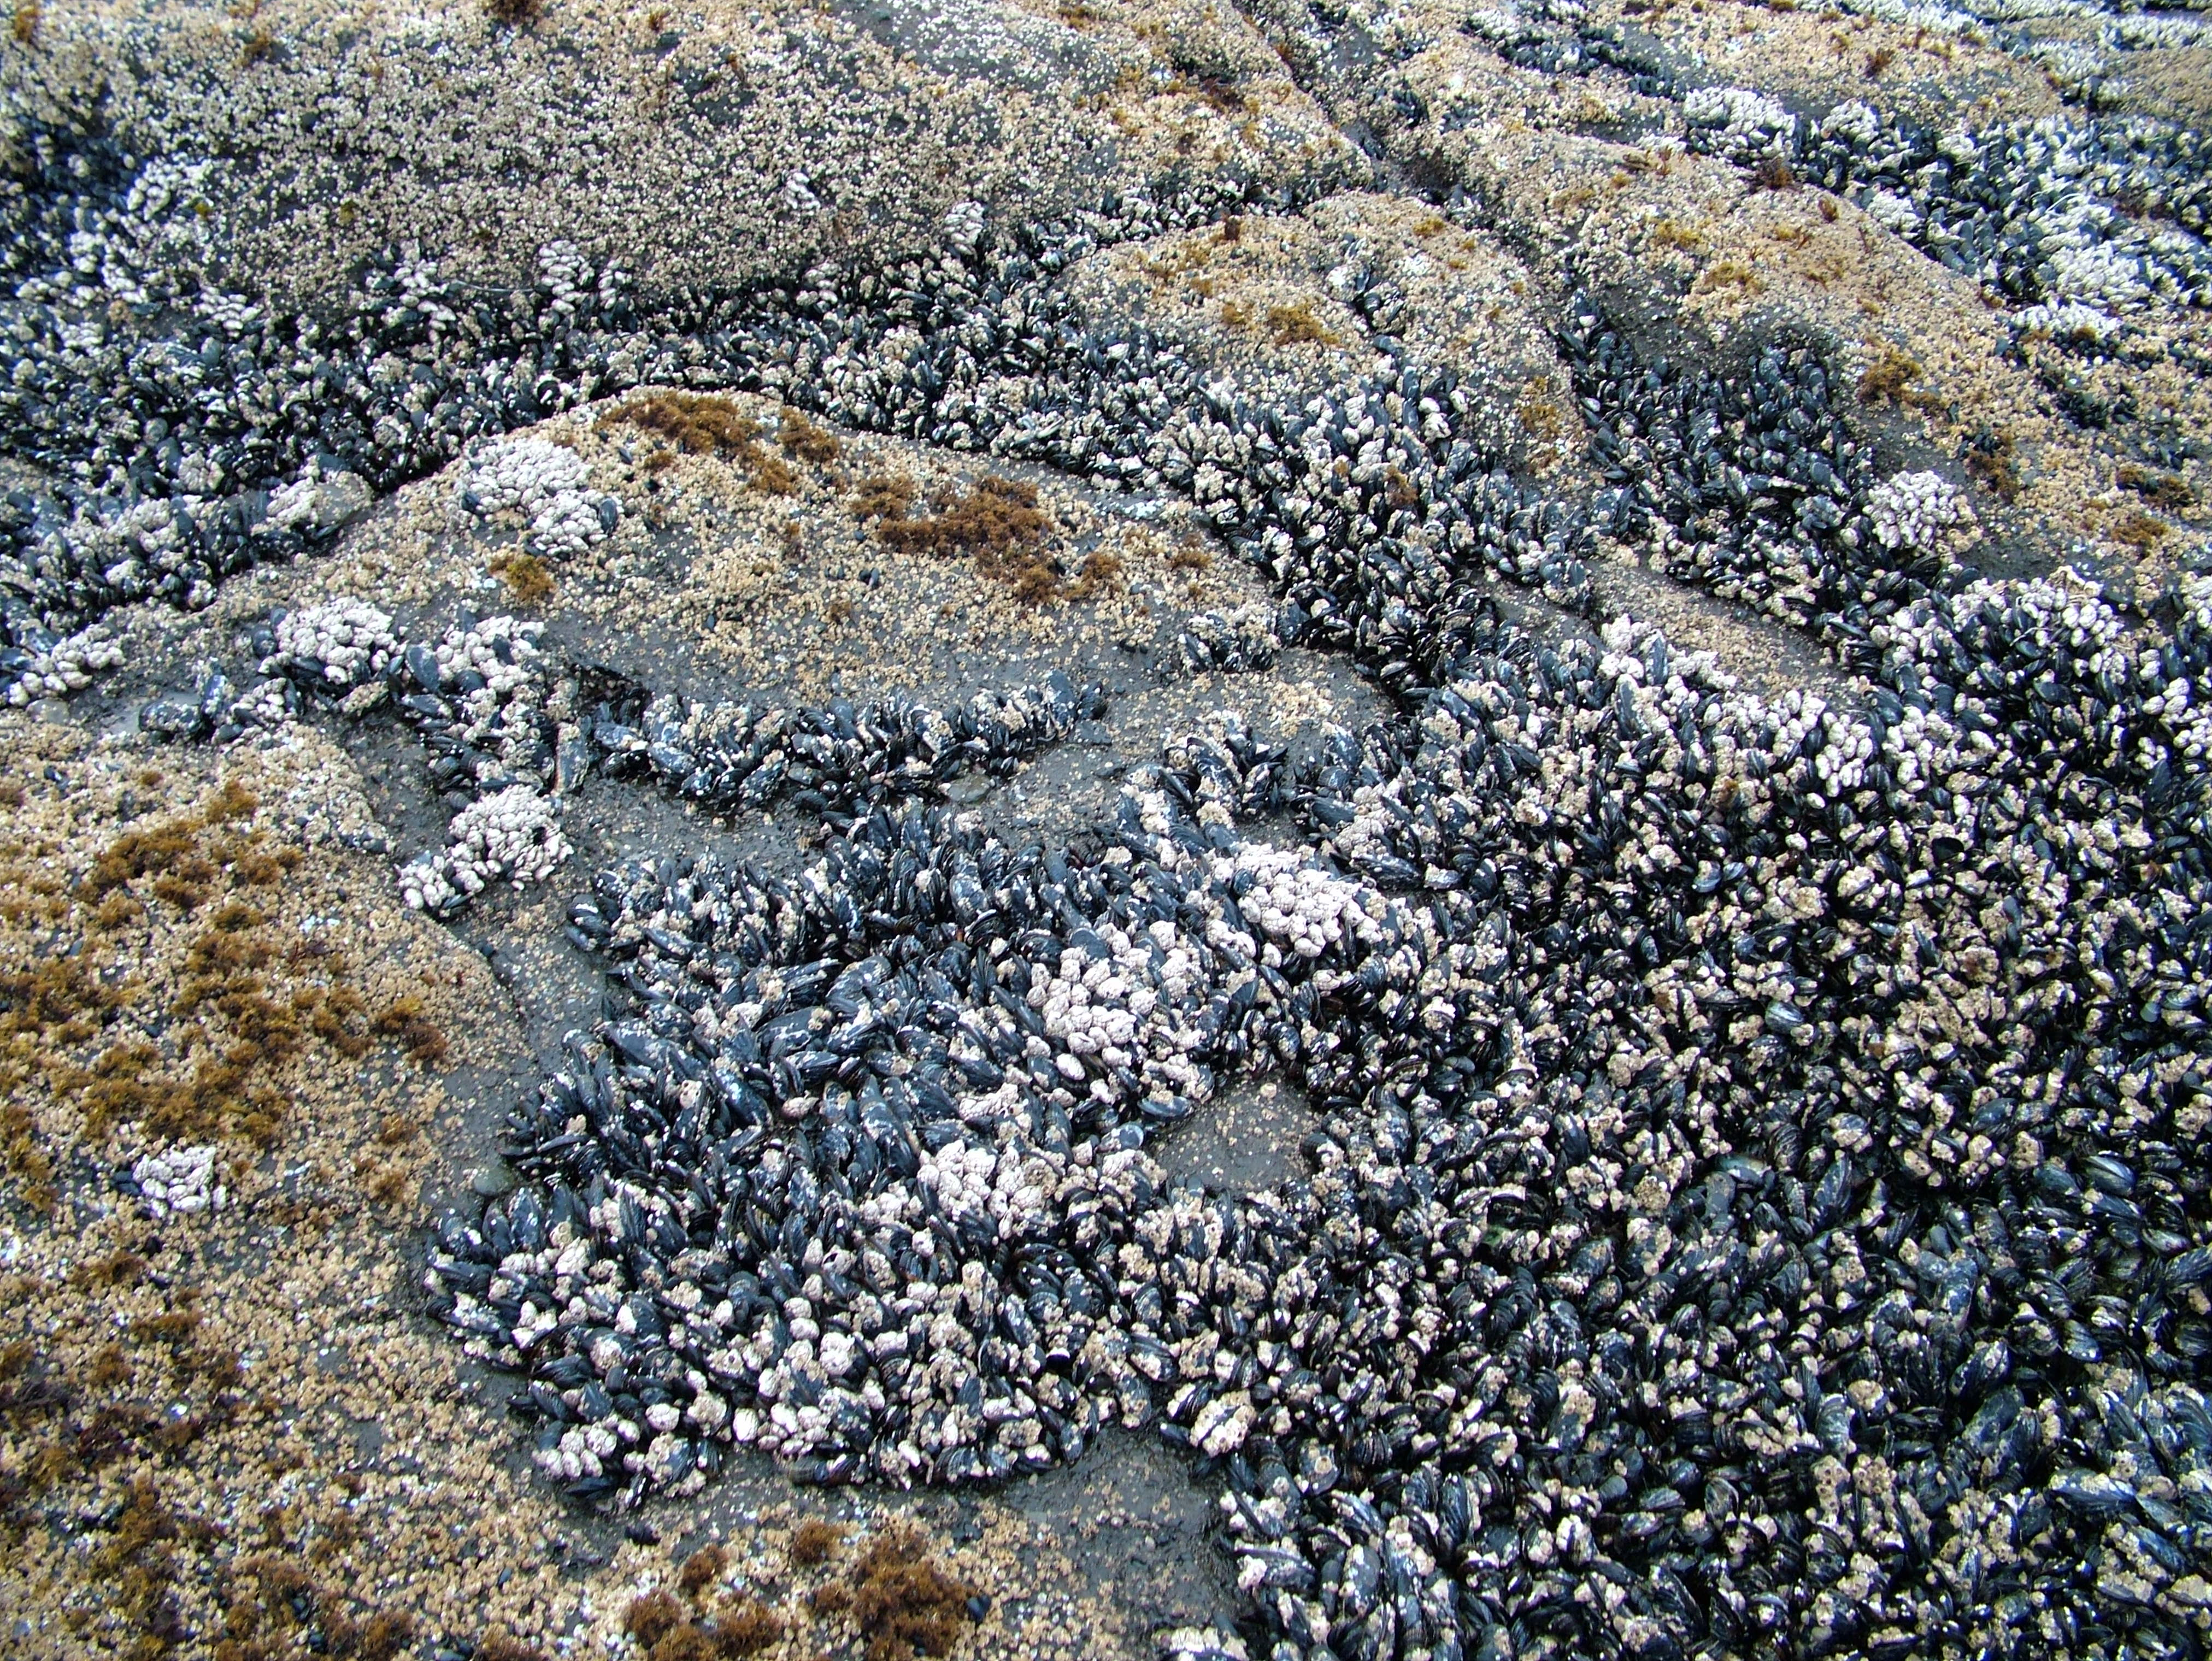
\includegraphics[height=0.7\textheight]{Figs/barnacles}
    \end{center}

\end{frame}

%------------------------------

{
\usebackgroundtemplate{}
\begin{frame}

	\pagecolor{BDQC1st}
	\color{white}

	\LARGE{\textit{Exercise}}

\end{frame}
}

%------------------------------

\begin{frame}[fragile]{Spatially implicit metapopulation dynamics}

    \begin{verbatim}
        DEFINE vector of J patches
        FOR time steps
            Compute occupancy p
            FOR patch x
                IF presence[x] = 0 
                    IF rand < cp
                        presence[x] = 1
                ELSE rand < e
                        presence[x] = 0
    \end{verbatim}

    \begin{enumerate}
        \item Run simuations with e = 0.2 and c = 0.3
        \item What happens with J = 1000, J = 100, J = 10 ?
    \end{enumerate}
\end{frame}

%------------------------------

{
\usebackgroundtemplate{}
\begin{frame}

	\pagecolor{BDQC1st}
	\color{white}

	\LARGE{\textit{Theory}}

\end{frame}
}

%------------------------------

\begin{frame}{Patch}

	\begin{columns}
		\begin{column}{0.5\textwidth}
            \textbf{Definition :} a discrete area of suitable habitat that can support a local breeding population, separated from other similar areas by unsuitable matrix territory where individuals cannot permanently live
		\end{column}
%----
		\begin{column}{0.5\textwidth}	
            \begin{center}
                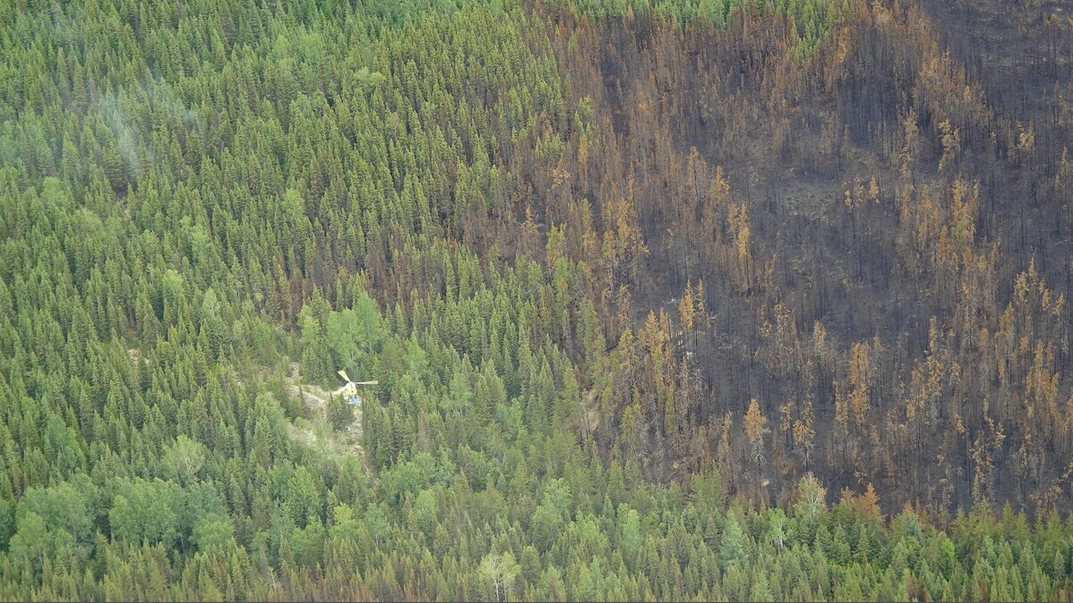
\includegraphics[height=0.4\textheight]{Figs/fire}
            \end{center}
		\end{column}				
	\end{columns} 

\end{frame}

%------------------------------

\begin{frame}{Scale-dependence}

    \begin{center}
        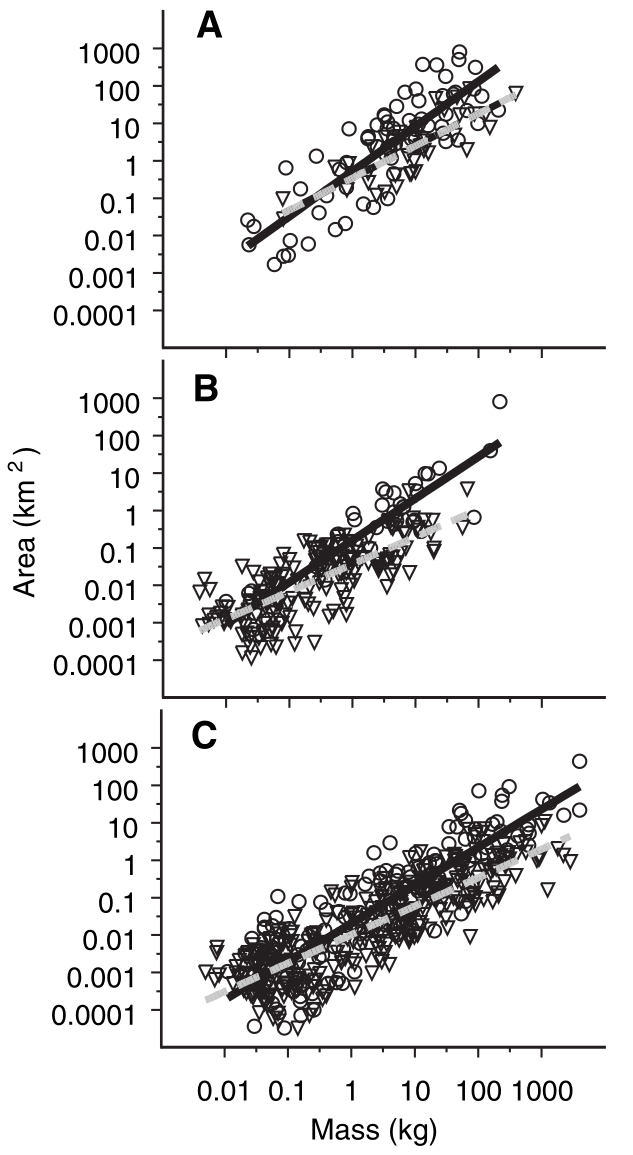
\includegraphics[height=0.7\textheight]{Figs/jetz2004}\\
        \footnotesize Jetz et al. 2004. Science.
    \end{center}

\end{frame}

%------------------------------

\begin{frame}{Patch}{Colonization}

	\begin{columns}
		\begin{column}{0.5\textwidth}
            \begin{center}
                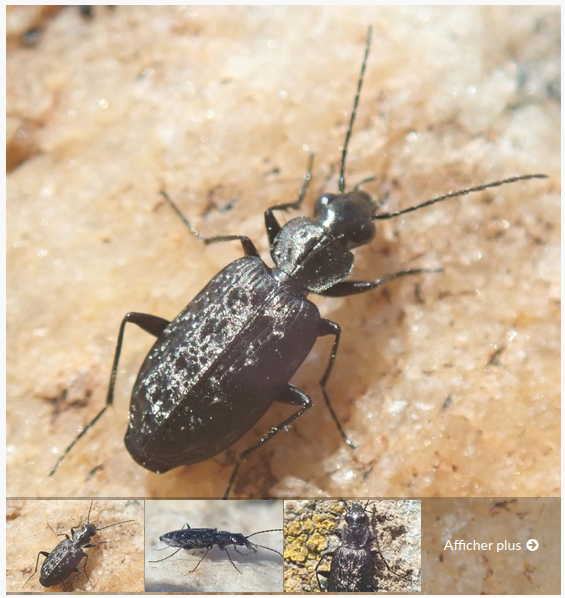
\includegraphics[height=0.5\textheight]{Figs/carabidae}
            \end{center}
		\end{column}
%----
		\begin{column}{0.5\textwidth}
            \begin{center}
                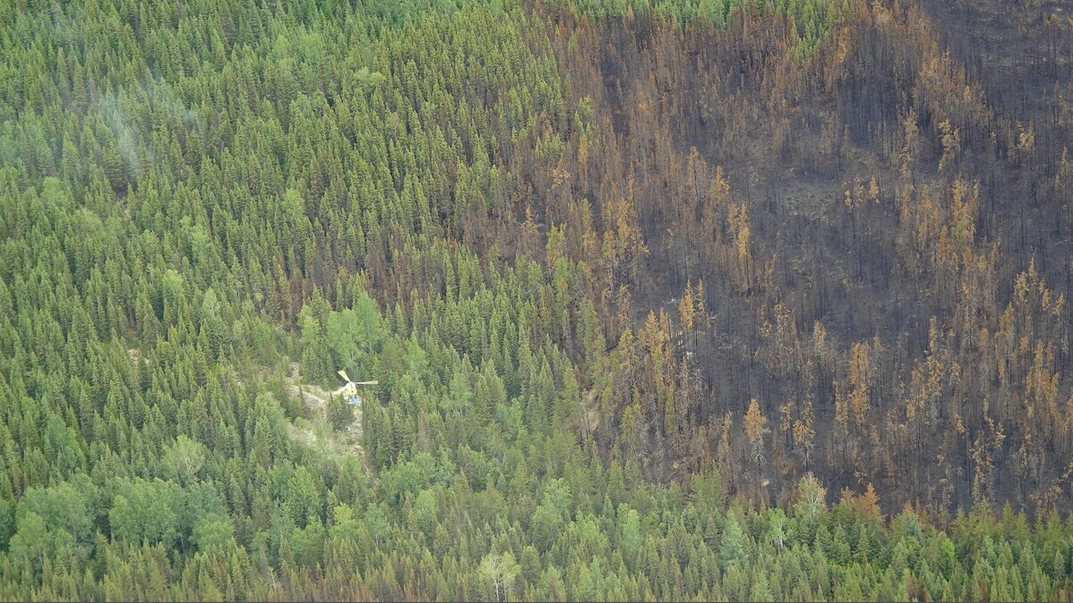
\includegraphics[height=0.4\textheight]{Figs/fire}
            \end{center}
		\end{column}
	\end{columns}

\end{frame}

%------------------------------

\begin{frame}{Patch}{Colonization}

	\begin{columns}
		\begin{column}{0.5\textwidth}
            \begin{center}
                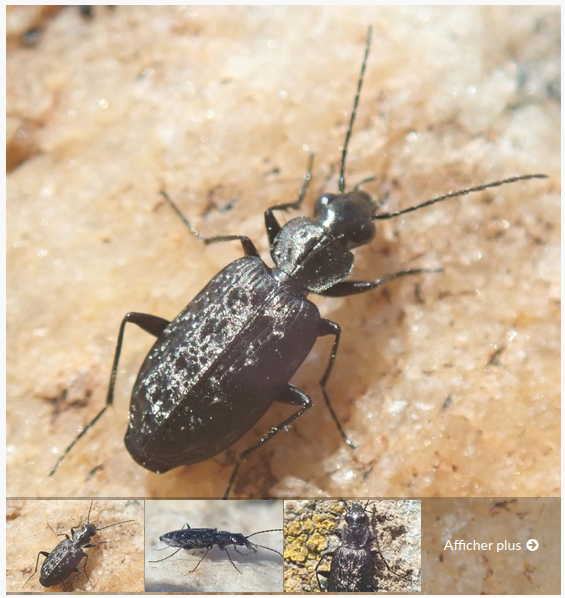
\includegraphics[height=0.5\textheight]{Figs/carabidae}
            \end{center}
		\end{column}
%----
		\begin{column}{0.5\textwidth}	
            \begin{itemize}
                \item Dispersal 
                \item Find empty patches
                \item Establishment
                \item Population growth
            \end{itemize}
		\end{column}				
	\end{columns} 

\end{frame}

%------------------------------

\begin{frame}{Patch}{Extinction}

	\begin{columns}
		\begin{column}{0.5\textwidth}
            \begin{center}
                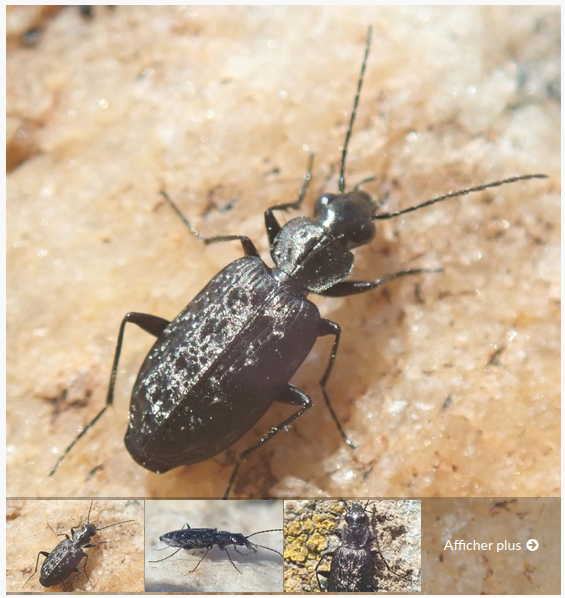
\includegraphics[height=0.5\textheight]{Figs/carabidae}
            \end{center}
		\end{column}
%----
		\begin{column}{0.5\textwidth}	
            \begin{itemize}
                \item Demographic stochasticity
                \item Selection
                \item Disturbance
            \end{itemize}
		\end{column}				
	\end{columns} 

\end{frame}

%------------------------------

\begin{frame}{Combining processes}

    \begin{center}
    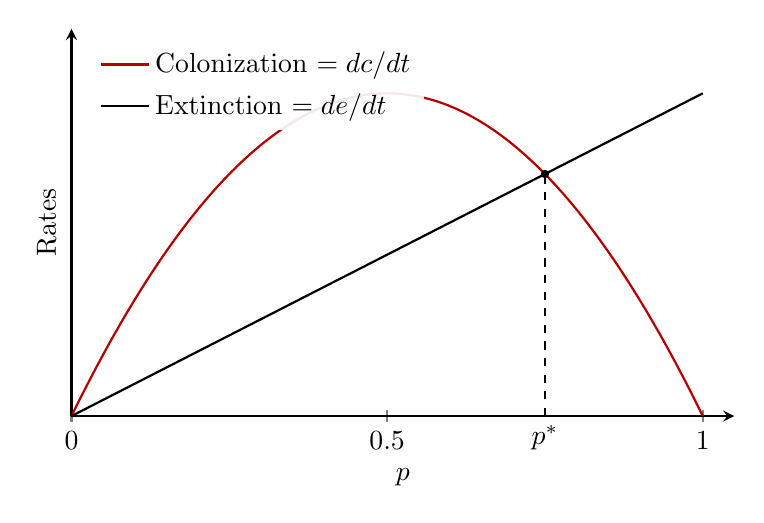
\begin{tikzpicture}
        \begin{axis}[
            width=10cm, height=6.5cm,
            xlabel={$p$}, ylabel={Rates},
            xmin=0, xmax=1.05, ymin=0, ymax=0.30,
            xtick={0,0.5,1}, ytick=\empty,
            axis lines=left,
            axis line style={-stealth, thick},
            tick style={thick},
            label style={font=\normalsize},
            tick label style={font=\normalsize},
            legend style={
                draw=none, fill=white, fill opacity=0.9,
                text opacity=1,
                font=\normalsize,
                at={(0.03,0.97)}, anchor=north west,
                row sep=2pt,
            },
            legend cell align={left},
            clip=false,
        ]
            % Colonization : dc/dt = p(1-p)
            \addplot[thick, red!70!black, domain=0:1, samples=100] {x*(1-x)};
            \addlegendentry{Colonization $=dc/dt$}
            % Extinction : de/dt = ep, with e = 0.25
            \addplot[thick, black, domain=0:1, samples=2] {0.25*x};
            \addlegendentry{Extinction $=de/dt$}
            % Equilibrium p* = 1 - e
            \addplot[only marks, mark=*, mark size=1.3pt, black, forget plot] coordinates {(0.75,0.1875)};
            \draw[dashed] (axis cs:0.75,0) -- (axis cs:0.75,0.1875);
            \node[anchor=north] at (axis cs:0.75,0) {\normalsize $p^*$};
        \end{axis}
    \end{tikzpicture}
    \end{center}

\end{frame}

%------------------------------

\begin{frame}{Levins model}

    The Levins metapopulation model describes the proportion $p$ of occupied patches in a landscape as :

    \keyeq{\frac{dp}{dt} = \underbrace{cp}_{\text{propagules}}\underbrace{(1-p)}_{\text{empty patches}} - \underbrace{ep}_{\text{extinction}}}

\end{frame}

%------------------------------

\begin{frame}{Levins model}{Persistence}

    The fundamental result of metapopulation theory is that persistence requires :

    \keyeq{c>e}
    
\end{frame}

%------------------------------

\begin{frame}{Levins model}{Equilibrium}

    Time dynamics follow asymptotic curve :

    \keyeq{p(t) = \frac{1}{\dfrac{1}{p_0}\exp(-(c-e)t)+\dfrac{c}{c-e}\left(1-\exp(-(c-e)t)\right)}}

    With equilibrium :

    \keyeq{p^*= 1 - \frac{e}{c}}
    
\end{frame}

%------------------------------

\begin{frame}{Levins model}{Interpretation}

    \begin{itemize}
        \item Occupancy increases non-linearly with colonization 
        \item Occupancy decreases linearly with extinction
        \item Dynamics are globally stable
        \item Asymptotic growth
        \item Variability depends on the number of patches
    \end{itemize}
    
\end{frame}

%------------------------------

\begin{frame}{Levins model}{Assumptions}

    \begin{itemize}
        \item Discrete landscape
        \item Separation of time scales 
        \item Infinite number of patches
        \item All patches are identical
        \item Landscape is constant over time
        \item Surrounding matrix is inhospitable
        \item Independence of $c$ and $e$
        \item Global dispersal 
    \end{itemize}
    
\end{frame}

%------------------------------

{
\usebackgroundtemplate{}
\begin{frame}

	\pagecolor{BDQC1st}
	\color{white}

	\LARGE{\textit{Exercise}}

\end{frame}
}

%------------------------------

\begin{frame}[fragile]{Spatially explicit dynamics}

    \begin{verbatim}
        DEFINE presence     # vector of J patches
        DEFINE XY           # array of spatial coordinates
        DEFINE ConMat       # Connectivity matrix
        DEFINE Nmax         # Number of nearest neighbors
        FOR time steps            
            FOR patch x
                IF presence[x] = 0 
                    ConPop = ConMat%*%presence / Nmax
                    IF rand < cp 
                        presence[x] = 1
                ELSE rand < e
                        presence[x] = 0
    \end{verbatim}

\end{frame}

%------------------------------

\begin{frame}[fragile]{Spatially explicit dynamics}{Questions}

    \begin{enumerate}
        \item Run simuations with e = 0.2 and c = 0.3
        \item What happens with J = 1000, J = 100, J = 10 ?
        \item \textbf{Advanced :} compare with random connectivity
    \end{enumerate}

\end{frame}

%------------------------------

{
\usebackgroundtemplate{}
\begin{frame}

	\pagecolor{BDQC1st}
	\color{white}

	\LARGE{\textit{Back to theory}}

\end{frame}
}

%------------------------------

\begin{frame}{Pair approximation}

    \begin{itemize}
        \item Consider patches are aligned along a circle
        \item Dispersal only occurs between adjacent patches
        \item We model the dynamics of pairs of patches
    \end{itemize}
    
\end{frame}

%------------------------------

\begin{frame}{Pair approximation}{Model}

    We have a set of three differential equations :

    \keyeqs{
    \frac{dp_{EE}}{dt} &= 2ep_{OE}-cp_{EE}\left(\frac{p_{OE}}{p_{OE}+p_{OO}}\right)\\[4pt]
    \frac{dp_{OE}}{dt} &= \frac{c}{2}p_{EE}\left(\frac{p_{OE}}{p_{OE}+p_{OO}}\right)+ep_{OO}-\left[e+\frac{c}{2}\left(1+\frac{p_{OE}}{p_{OE}+p_{OO}}\right)\right]p_{OE}\\[4pt]
    \frac{dp_{OO}}{dt} &= c\left(1+\frac{p_{OE}}{p_{OE}+p_{OO}}\right)p_{OE}-2ep_{OO}
    }
\end{frame}

%------------------------------

\begin{frame}{Pair approximation}{Solution}

    Which yields the equilibrium metapopilation occupancy :

    \keyeq{p = \frac{1-2(e/c)}{1-(e/c)}}
\end{frame}

%------------------------------

\begin{frame}{Pair approximation}{Autocorrelation}

    Local dispersal has for result that pairs of patches tend to be more similar than with global dispersal. 

    The spatial autocorrelation in this model is :

    \keyeq{\rho = \frac{e}{c}}

    And we can re-arrange equilibrium solution as :

    \keyeq{p^* = 1 - \frac{e}{c}\frac{1}{1-\rho}}

\end{frame}

%------------------------------

\begin{frame}{Pair approximation}{Interpretation}

    \begin{itemize}
        \item Spatially explicit dispersal genetes positive autocorrelation 
        \item Autocorrelation declines with increasing colonization     
        \item Spatially explicit dispersal reduces equilibrium occupancy 
    \end{itemize}
    
    The [very] important notion of dispersal limitation becomes clear : ecological conditions may result in situations where a species is absent from a location where it should be. 

\end{frame}

%------------------------------

\begin{frame}{Habitat destruction}

    The standard Levins model assumes that the entire set of suitable patches is available for colonization. 

    Habitat destruction $D$ can be introduced as follows :

    \keyeq{\frac{dp}{dt} = cp(1 - D - p) - ep}

\end{frame}

%------------------------------

\begin{frame}{Habitat destruction}

    Persistence now requires that :

    \keyeq{c(1-D)>e}

    Which means that a species may go extinct, even if $c>e$ and that there are remaining suitable habitats.

\end{frame}

%------------------------------

\begin{frame}{Habitat destruction}{Spatially explicit}

	\begin{columns}
		\begin{column}{0.5\textwidth}
            \begin{center}
                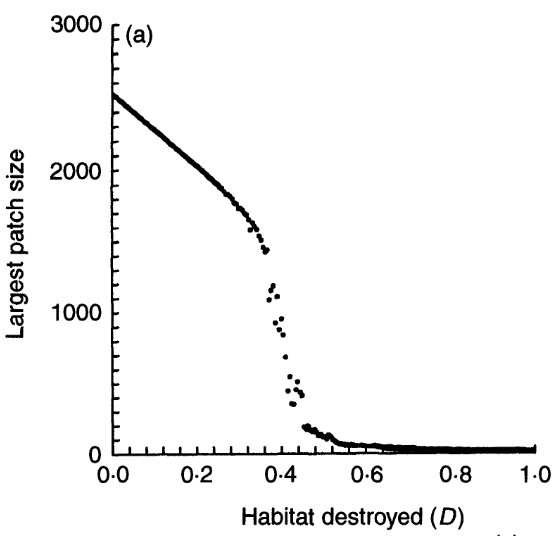
\includegraphics[height=0.5\textheight]{Figs/bascompte1996a}
            \end{center}
		\end{column}
%----
		\begin{column}{0.5\textwidth}	
            \begin{center}
                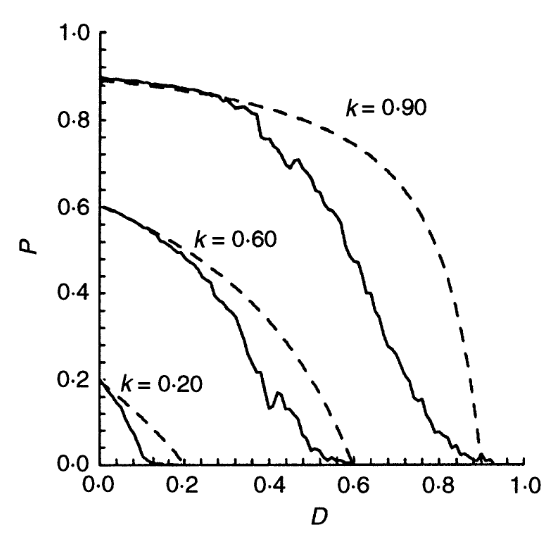
\includegraphics[height=0.5\textheight]{Figs/bascompte1996b}
            \end{center}
		\end{column}				
	\end{columns} 

    Spatially explicit dynamics magnifies the effect of habitat destruction

\end{frame}

%------------------------------
%------------------------------
%------------------------------
\end{document}
